\section{Marching cubes}
\label{sec:marching_cubes}
The geometry in DSMC is represented as voxels as we discussed in section \ref{sec:dsmc_complex_geometries}. They form a scalar field with values zero for empty voxels and non-zero for filled voxels. The surface of the geometry is where the values of the scalar field \textit{changes} from zero to a non-zero value. This defines the \textit{iso-surface}, i.e. a surface where all the values on one side are zero, and non-zero on the other side. If we find a way to visualize this iso-surface, it will coincide with where the DSMC particles collide. We then need to create some primitives (in this case triangles) that are connected to each other, forming a the full iso-surface. Such an algorithm exists and is called \textit{marching cubes}.

Marching cubes is an algorithm used to generate a set of connected triangles from the iso-surface of a scalar field. The method was presented in a paper published in 1987 and has been widely used in medical visualizations of CT and MRI scans \cite{wiki:marching_cubes}. Assuming that the scalar field is discretized in space, each point - vertex in our case - has a value larger or larger than some chosen iso-value. Given a cube consisting of eight of these vertices, there exists $2^{8}=256$ unique combinations (each vertex has two possibilities). Because of symmetries (a cube with only one vertex being larger than the iso-value has through rotations 8 different configurations that really are the same configuration), this set can be reduced to 15. In figure \ref{fig:vis_marching_cubes}, we see the 15 unique configurations and the corresponding triangles in each configuration.
\begin{figure}[htb]
\begin{center}
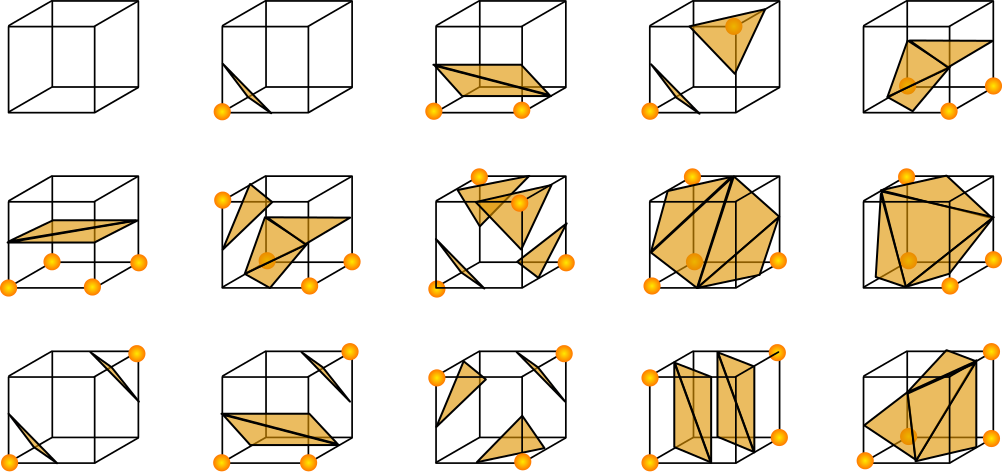
\includegraphics[width=0.8\textwidth, trim=0cm 0cm 0cm 0cm, clip]{visualization/figures/marching_cubes.png}
\end{center}
\caption{A cube consisting of eight vertices. Given that each vertex can have a value smaller or larger than some given iso-value, the cube has has $2^8=256$ different combinations. This number can, as we see here, be reduced to 15 due to symmetries. An iso-surface on a scalar field can then be generated as renderable triangles with this technique. Image from \url{http://en.wikipedia.org/wiki/File:MarchingCubes.svg}, accessed 20 March, 2014.}
\label{fig:vis_marching_cubes}
\end{figure}
For a given cube, the 8 vertex values (one or zero) can be represented as the bits in an 8-bit integer. The final value of this integer is then the index of a precomputed table containing a list of all triangles needed for that configuration.

The original authors thought the 15 combinations would be enough, but it turns out that with these 15 configurations, there exists cases where the surface gets holes - it is not topologically correct. This problem was solved in 1995 by using a larger set with 33 unique configurations which spans out the full configuration space \cite{chernyaev1995marching}. We have used a precomputed table with 256 configurations made from this basis of 33 elements. Each vertex is part of at least one triangle. We can then compute the normal vector per vertex as an average of the normal vectors of all triangles it is a part of. This enables the fragment shader to get interpolated normal vectors per vertex giving beautiful, smooth shadows as we can see in figure \ref{fig:vis_marching_cubes_1}. Surfaces having a normal vector pointing towards the camera have maximum light intensity. All other surfaces will have reduced light intensity proportional to the dot product between the normalized camera-to-object vector and the normal vector.

Since the geometry in DSMC model is described by a scalar field with values zero, one and two, we can choose iso-value of one and use the marching cube algorithm to generate triangles we can render on the GPU. The set of triangles is uploaded to the graphics card as a VBO and is rendered with a simple draw call. In figure \ref{fig:vis_marching_cubes_1}, we have rendered the packed spheres we studied in section \ref{sec:dsmc_packed_spheres_results} with the marching cubes algorithm. Here we used $256\times256\times256$ voxels obeying periodic symmetry in all directions. Two overlapping spheres will have a smooth, shared surface as we see in the top of the figure.

\begin{figure}[htb]
\begin{center}
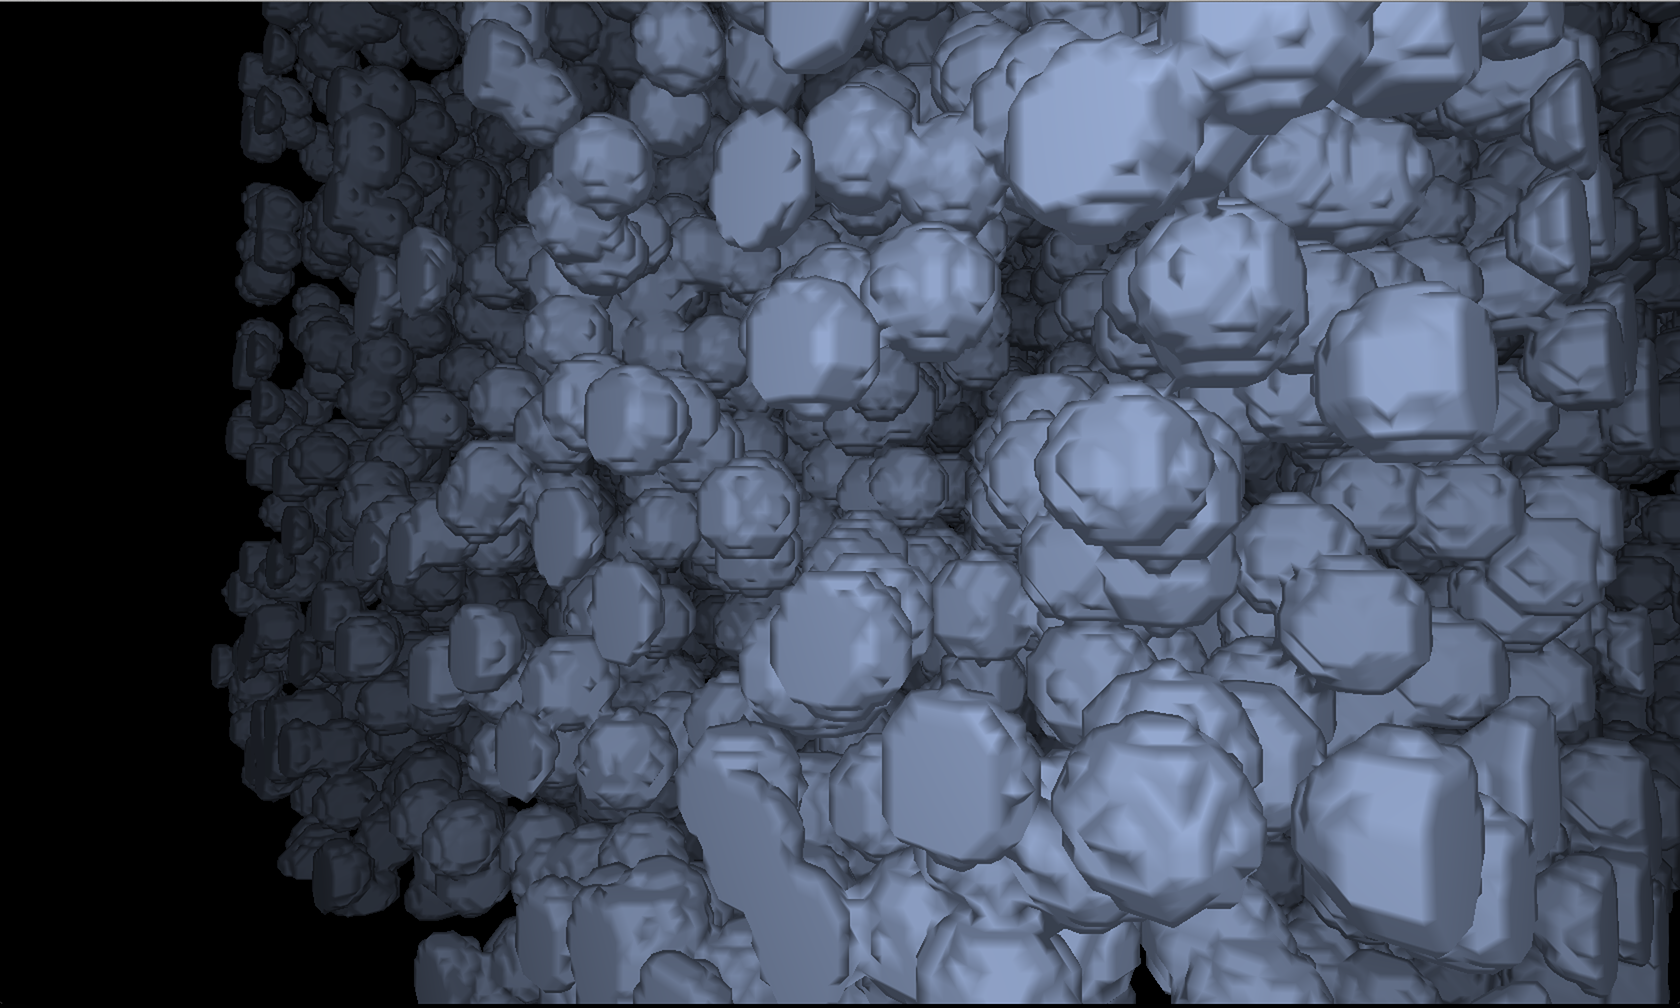
\includegraphics[width=\textwidth, trim=0cm 0cm 0cm 0cm, clip]{visualization/figures/marching_cubes_spheres_1.png}
\end{center}
\caption{Randomly packed spheres in DSMC visualized with the marching cubes algorithm. The geometry is made up by $256\times256\times256$ voxels obeying periodic symmetry in all directions. In the top of the figure, we see two how marching cubes elegantly renders two overlapping spheres. Normal vectors are computed for each vertex by averaging the normal vectors of all the triangles it is a part of. This enables the fragment shader to get interpolated normal vectors per vertex giving beautiful, smooth shadows.}
\label{fig:vis_marching_cubes_1}
\end{figure}